%This is Janet's for the NSF.
\documentclass[11pt]{article}
\usepackage{graphicx,color}
\usepackage{rotating}
\usepackage{epsfig,graphics,rotate,color}
\usepackage{wrapfig}
\topmargin 0pt
\advance \topmargin by -\headheight
\advance \topmargin by -\headsep
\textheight 8.9in     
\oddsidemargin 0pt
\evensidemargin \oddsidemargin
\marginparwidth 0.5in
\textwidth 6.5in

%This is mine for changing the font.
\usepackage[T1]{fontenc}
\usepackage{times}
 \usepackage{hyperref}

%This is for NSF style
\bibliographystyle{utphys}

\begin{document} 
%Do this myself
%\begin{center}
%\Large{Next-Generation Liquid-Scintillator-Based Detectors: \\ Quantums Dots and Picosecond Timing}\\[0.25cm]
%\large{Lindley Winslow,  \today}\\[0.25cm]
%\end{center}
\noindent
Dear JINST Editors, \\

In the following draft we have attempted to address the excellent comments of the referees and below we provide some additional information. In some areas we would like to limit the scope of the work proposed by the referees. We envisioned this paper as a proof-of-principle. The reconstruction of the direction of low energy ($\sim$1 MeV) electrons in a liquid scintillator detector has never been shown before. In this paper, we wanted to show the following: the scintillation/Cherenkov separation was possible, the parameters of a detector that were important to this separation, and finally that Cherenkov reconstruction techniques would work in idealized situations. We are now working on at least two follow-up papers. The first is a detailed study of  reconstruction in more realistic scenarios. The second is a $0\nu\beta\beta$  experiment proposal where the detailed background reduction factors and sensitivity to new physics are presented, SuperNEMO has a similar paper but nothing similar exists for scintillator detectors since a directional signal has not been considered for them in the past.  Finally, we will be having a turnover of personnel so this paper provides an excellent summary of their work.\\ 

\noindent
The following is a more detailed response to the referees' comments.\\ 

\noindent
Thank you,\\ 
Lindley Winslow for the authors
\\
\\
\noindent
{\bf Response to Referee 1}\\
Page 1: \\
Liquid scintillators detectors quote their resolution in terms of  $\sim$5\%$/\sqrt{E(MeV)}$. We have updated the text to make that more clear. \\ \\
Rewrote introduction to include NEXT/SuperNEMO and to be more clear about the energy resolution issues and our approach to this paper. \\ \\
Defined PPO earlier.\\

\noindent
Page 3: \\
Added some example values for the equations.\\ \\
There is one referee comment here that we did not know how to interpret, {\it This case is shown in Fig.1.
->Indicating the direction of the electrons should not harm.}\\ \\
Changed the wording about the Q-value and the background considerations. \\ \\


\noindent
Page 4: \\
Also added here some reference values for the cutoff wavelength etc. as requested. \\ \\
We have added a more detailed explanation on why optical scattering can be neglected and a detailed reference. In Fig.~\ref{scatt} below we also show the simulation results with and without optical scattering for reference. In the simulation without scattering a ``pure" attenuation length is used so photons are simply absorbed and disappear from the simulation, therefore when scattering is turned on more photons reach the sphere. The timing distribution gains a small tail at longer times as is expected.\\ \\
We fixed the wording for the explanation of the QE values.\\ \\
We added some text explaining why 5~MeV is good for evaluating the technique.\\ \\
We added the distance between the start and stop points. As can be seen in Fig.~\ref{truthscatt}, the scattering angles are small until the electron falls below Cherenkov threshold, therefore the light emitted encodes the emission direction of the primary electron.\\ \\


\begin{figure}
        \begin{center}
        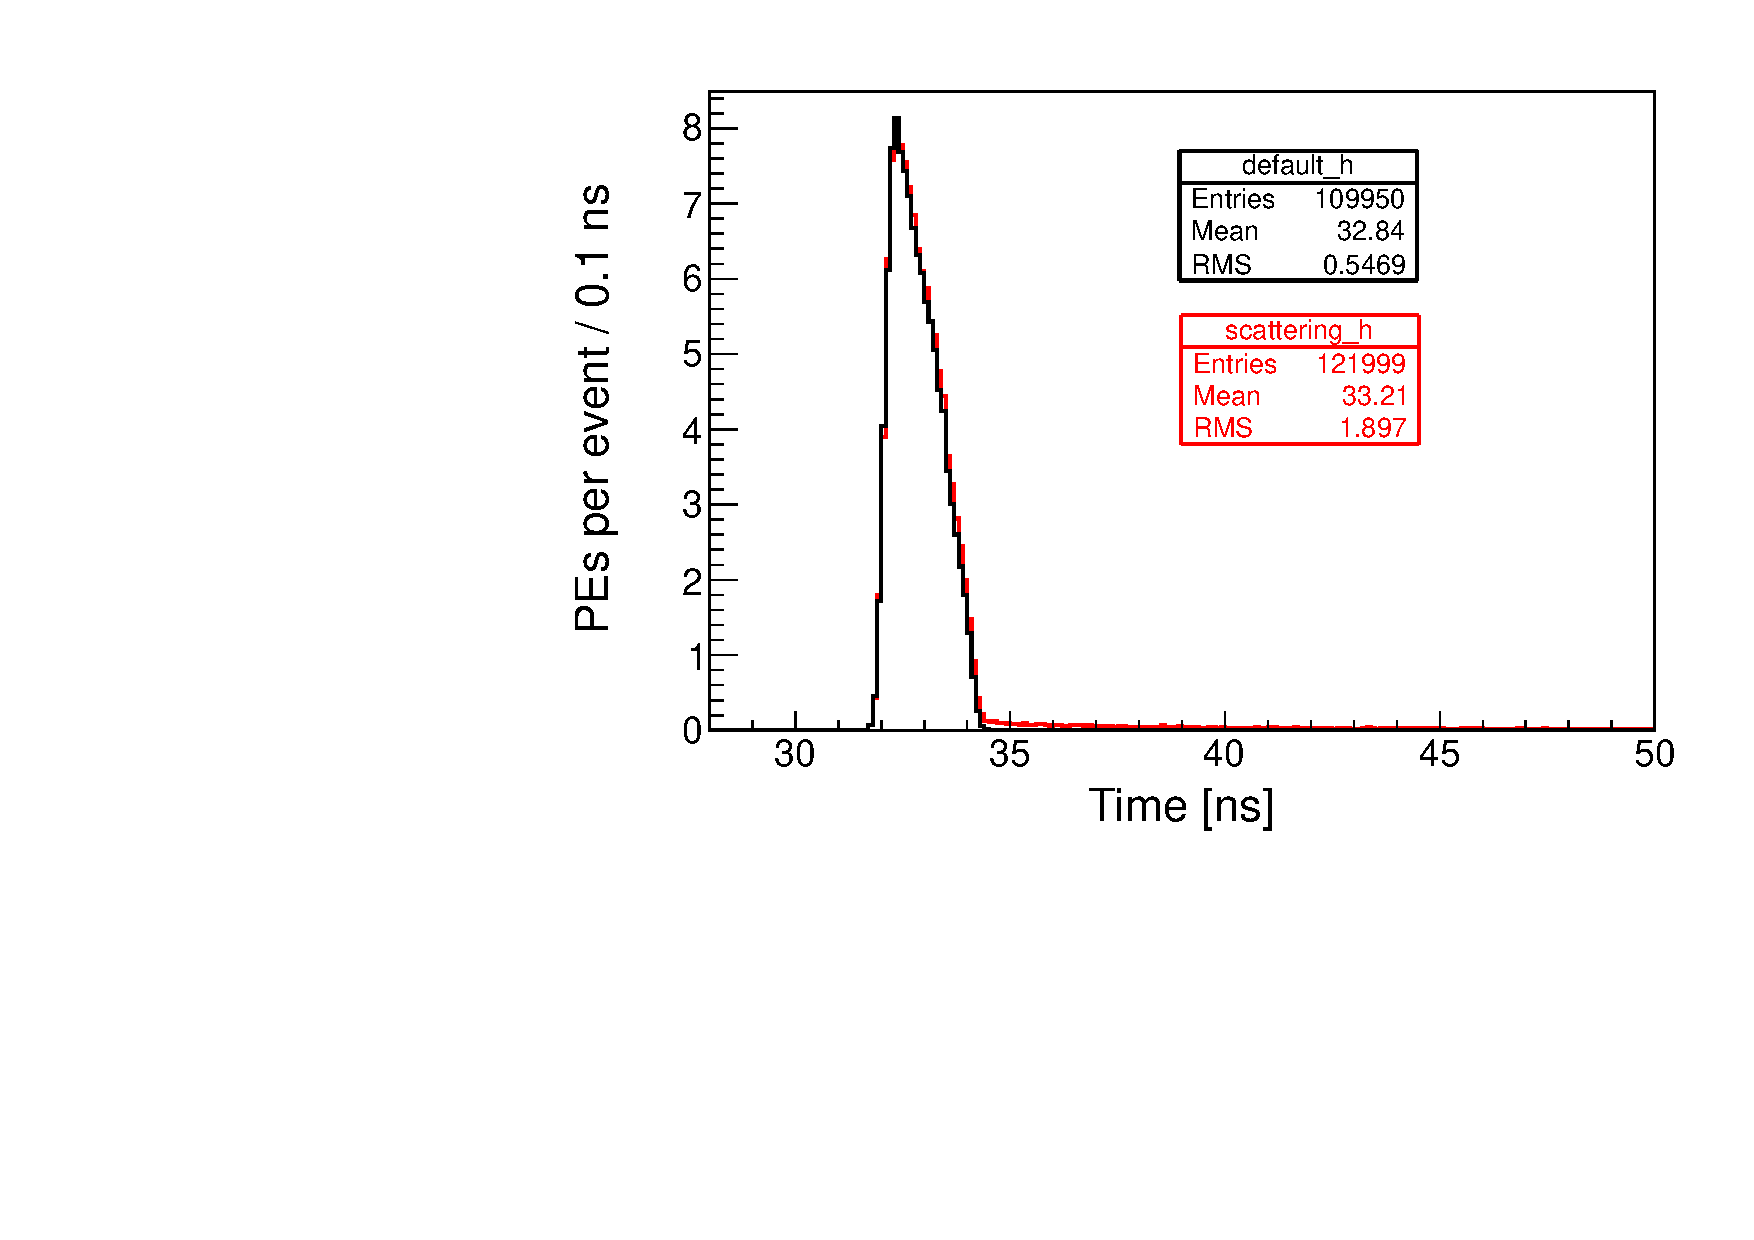
\includegraphics[scale=0.40]{Cerenkov_PEs_scattering_comparison.pdf} 
         \caption{The arrival time of Cherenkov light with (red) and without scattering (black).\label{scatt}}
        \end{center}
\end{figure}


\noindent
Page 5: \\
We rephrased the discussion of the energy transfer between solvent and solute.\\ \\
We updated the citations for the LAPPDs to more recent ones.\\ \\

\noindent
Page 6: \\
We have added a reference to the Geant4 standard electron physics list.  The main request of the referee is to see Fig. 3 as a function of the electron path. We are not setup to easily extract that information. Instead we point them to the data in Fig.~\ref{truthscatt} and we note again that the electron scattering is small during the time the electron is above Cherenkov threshold. In addition, we have remade Fig. 3 with all three energies and the Cherenkov structure is clear down to 1.4~MeV.

\begin{figure}
        \begin{center}
        \includegraphics[scale=0.50]{1p4_MeV_Direction_to_Stop.pdf} 
        \includegraphics[scale=0.50]{1p4_MeV_Direction_to_c_threshold_point.pdf} 
        \includegraphics[scale=0.50]{1p4MeV_direction_of_last_step_h.pdf} 
         \caption[]{Truth scattering data.\label{truthscatt}}
        \end{center}
\end{figure}

\noindent
Page 7-8: \\
We would like to leave the sections on scintillator in for completeness.\\ \\

\noindent
Page 9: \\
Added reconstruction plots for all energies and now note that the p$_x$ distribution is the $cos\theta$ distribution. \\ \\
The referee correctly notes that the vertex resolution is a sizable effect, so our use of the truth timing information is a non-negligible simplification. The effect is 0.15~s for the 3cm resolution. Eventually, we should simultaneously reconstruct the direction and vertex. This also addresses the issue of direction reconstruction in other sections of the detector. {\bf Should I add more here about our logic in neglecting this effect for this paper.  Since we are putting in the TTS smearing by hand,  we could simply double the transit time spread smearing we are using. We were interested in whether timing on the order of 0.1~ns, compared to the standard 1~ns, would allow us to reconstruct direction.}\\ \\
We now show the $cos\theta$ distribution for all energies. Fig.~7  is nice as you can see the performance of the reconstruction and extrapolate to higher or lower energies. For reference,  the Cherenkov threshold for  n(370nm)=1.465892 is 0.1879~MeV. This a logical choice of wavelength for defining the Cherenkov threshold since light produced below 370 nm will be absorbed before reaching the edge of the sphere since once again this is the absorption cutoff of the scintillator. \\ \\ 

\noindent
Conclusions:\\
We rewrote the conclusion to emphasize more that this is the first attempt to reconstruct direction in a liquid scintillator. \\ \\ \\ \\ 

\noindent
{\bf Response to Referee 2}\\

\begin{itemize}
\item The referee asked for more discussion on the possible sensitivity improvement. This is what we would like to work on next. It is obvious that it will but the magnitude requires a detailed sensitivity analysis and a better understanding of the final reconstruction performance. This is why we wanted to show it was possible first and then work on these more detailed and time intensive analyses. We have added some more discussion on the experience of other experiments as was requested by referee 1.
\item We agree 5~MeV is not interesting for $0\nu\beta\beta$, however it is interesting to neutrino-electron scattering interactions (also referred to in the title) and this allowed us to verify our simulation and reconstruction and then push to lower energies where lower photon statistics make the verification more difficult. In the reconstruction section we do present the results of lower energy.
\item  We agree that position dependence is going to be important. Our next step is to simultaneously reconstruct position and direction. A preliminary attempt  using all the photons to do the position reconstruction at 5~MeV showed no bias and a decrease in the resolution to 8.5~cm. The position reconstruction uncertainty is equivalent to a larger TTS smearing so our direction reconstruction results will degrade or improve depending on the vertex reconstruction. This is the content of a more detailed paper to follow.
\item The statistical fluctuations are a good point. We added discussion on this to accompany what was Fig.~7, the average $cos\theta$ plot.  {\bf I still need to address this, any suggestions?}
\end{itemize}

Most of the more detailed requests were addressed in the response to referee 1.  These are the ones unique to referee 2:

\begin{itemize}
\item Added reference for matter-antimatter asymmetry.
\item Added definition of x.
\item Clarified wording of a ``probable case", now dependent on model. We also added the reference to Boehm and Vogel.
\item Added discussion of how scattering at the sphere would affect the timing discussion.
\end{itemize}

{\bf \it This completes the comments of the referees.}

%Here is the bibliography
%\bibliography{QuantumDotWhitepaper} 
\end{document}  